\documentclass[tikz,border=5pt]{standalone}
\usepackage{tikz}
\usetikzlibrary{arrows.meta,positioning}

\begin{document}
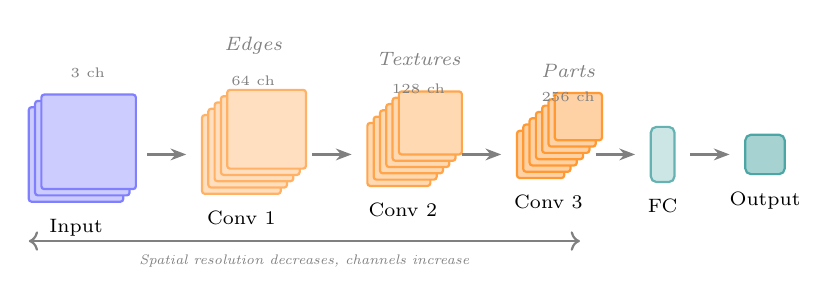
\begin{tikzpicture}[
    node distance=0.4cm,
    arrow/.style={-{Stealth[length=2mm]}, thick, gray},
    label/.style={font=\scriptsize, align=center},
    feature/.style={font=\scriptsize\itshape, text=gray, align=center}
]

% Input image (3 channels - RGB)
\foreach \i in {1,2,3} {
    \pgfmathsetmacro{\offset}{(\i-1)*0.08}
    \fill[blue!20, draw=blue!50, thick, rounded corners=1pt]
        (0+\offset, 0+\offset) rectangle ++(1.2, 1.2);
}
\node[below=0.1cm, font=\scriptsize] at (0.6, 0) {Input};
\node[above=0.1cm, font=\tiny, text=gray] at (0.75, 1.35) {3 ch};

% Arrow
\draw[arrow] (1.5, 0.6) -- (2.0, 0.6);

% Conv 1 (many channels, slightly smaller spatial)
\foreach \i in {1,...,5} {
    \pgfmathsetmacro{\offset}{(\i-1)*0.08}
    \fill[orange!25, draw=orange!60, thick, rounded corners=1pt]
        (2.2+\offset, 0.1+\offset) rectangle ++(1.0, 1.0);
}
\node[below=0.1cm, font=\scriptsize] at (2.7, 0.1) {Conv 1};
\node[above=0.1cm, font=\tiny, text=gray] at (2.85, 1.25) {64 ch};
\node[feature, above=0.5cm] at (2.85, 1.25) {Edges};

% Arrow
\draw[arrow] (3.6, 0.6) -- (4.1, 0.6);

% Conv 2 (more channels, smaller spatial)
\foreach \i in {1,...,6} {
    \pgfmathsetmacro{\offset}{(\i-1)*0.08}
    \fill[orange!30, draw=orange!70, thick, rounded corners=1pt]
        (4.3+\offset, 0.2+\offset) rectangle ++(0.8, 0.8);
}
\node[below=0.1cm, font=\scriptsize] at (4.75, 0.2) {Conv 2};
\node[above=0.1cm, font=\tiny, text=gray] at (4.95, 1.15) {128 ch};
\node[feature, above=0.45cm] at (4.95, 1.15) {Textures};

% Arrow
\draw[arrow] (5.5, 0.6) -- (6.0, 0.6);

% Conv 3 (even more channels, even smaller spatial)
\foreach \i in {1,...,7} {
    \pgfmathsetmacro{\offset}{(\i-1)*0.08}
    \fill[orange!35, draw=orange!80, thick, rounded corners=1pt]
        (6.2+\offset, 0.3+\offset) rectangle ++(0.6, 0.6);
}
\node[below=0.1cm, font=\scriptsize] at (6.6, 0.3) {Conv 3};
\node[above=0.1cm, font=\tiny, text=gray] at (6.85, 1.05) {256 ch};
\node[feature, above=0.4cm] at (6.85, 1.05) {Parts};

% Arrow
\draw[arrow] (7.2, 0.6) -- (7.7, 0.6);

% Flatten + FC
\fill[teal!20, draw=teal!60, thick, rounded corners=2pt]
    (7.9, 0.25) rectangle ++(0.3, 0.7);
\node[below=0.1cm, font=\scriptsize] at (8.05, 0.25) {FC};

% Arrow
\draw[arrow] (8.4, 0.6) -- (8.9, 0.6);

% Output
\fill[teal!35, draw=teal!70, thick, rounded corners=2pt]
    (9.1, 0.35) rectangle ++(0.5, 0.5);
\node[below=0.1cm, font=\scriptsize] at (9.35, 0.35) {Output};

% Annotations at bottom
\draw[<->, gray, thick] (0, -0.5) -- (7.0, -0.5);
\node[font=\tiny\itshape, text=gray] at (3.5, -0.75) {Spatial resolution decreases, channels increase};

\end{tikzpicture}
\end{document}
